\documentclass[]{article}
\usepackage{lmodern}
\usepackage{amssymb,amsmath}
\usepackage{ifxetex,ifluatex}
\usepackage{fixltx2e} % provides \textsubscript
\ifnum 0\ifxetex 1\fi\ifluatex 1\fi=0 % if pdftex
  \usepackage[T1]{fontenc}
  \usepackage[utf8]{inputenc}
\else % if luatex or xelatex
  \ifxetex
    \usepackage{mathspec}
  \else
    \usepackage{fontspec}
  \fi
  \defaultfontfeatures{Ligatures=TeX,Scale=MatchLowercase}
\fi
% use upquote if available, for straight quotes in verbatim environments
\IfFileExists{upquote.sty}{\usepackage{upquote}}{}
% use microtype if available
\IfFileExists{microtype.sty}{%
\usepackage{microtype}
\UseMicrotypeSet[protrusion]{basicmath} % disable protrusion for tt fonts
}{}
\usepackage[margin=1in]{geometry}
\usepackage{hyperref}
\hypersetup{unicode=true,
            pdftitle={Supplementary material for The utility of spatial model-based estimators of unobserved bycatch: future or folly?},
            pdfauthor={Brian C. Stock1, Eric J. Ward2, James T. Thorson2, Jason E. Jannot2, Brice X. Semmens1},
            pdfborder={0 0 0},
            breaklinks=true}
\urlstyle{same}  % don't use monospace font for urls
\usepackage{graphicx,grffile}
\makeatletter
\def\maxwidth{\ifdim\Gin@nat@width>\linewidth\linewidth\else\Gin@nat@width\fi}
\def\maxheight{\ifdim\Gin@nat@height>\textheight\textheight\else\Gin@nat@height\fi}
\makeatother
% Scale images if necessary, so that they will not overflow the page
% margins by default, and it is still possible to overwrite the defaults
% using explicit options in \includegraphics[width, height, ...]{}
\setkeys{Gin}{width=\maxwidth,height=\maxheight,keepaspectratio}
\IfFileExists{parskip.sty}{%
\usepackage{parskip}
}{% else
\setlength{\parindent}{0pt}
\setlength{\parskip}{6pt plus 2pt minus 1pt}
}
\setlength{\emergencystretch}{3em}  % prevent overfull lines
\providecommand{\tightlist}{%
  \setlength{\itemsep}{0pt}\setlength{\parskip}{0pt}}
\setcounter{secnumdepth}{0}
% Redefines (sub)paragraphs to behave more like sections
\ifx\paragraph\undefined\else
\let\oldparagraph\paragraph
\renewcommand{\paragraph}[1]{\oldparagraph{#1}\mbox{}}
\fi
\ifx\subparagraph\undefined\else
\let\oldsubparagraph\subparagraph
\renewcommand{\subparagraph}[1]{\oldsubparagraph{#1}\mbox{}}
\fi

%%% Use protect on footnotes to avoid problems with footnotes in titles
\let\rmarkdownfootnote\footnote%
\def\footnote{\protect\rmarkdownfootnote}

%%% Change title format to be more compact
\usepackage{titling}

% Create subtitle command for use in maketitle
\newcommand{\subtitle}[1]{
  \posttitle{
    \begin{center}\large#1\end{center}
    }
}

\setlength{\droptitle}{-2em}

  \title{Supplementary material for `The utility of spatial model-based
estimators of unobserved bycatch: future or folly?'}
    \pretitle{\vspace{\droptitle}\centering\huge}
  \posttitle{\par}
    \author{Brian C. Stock\textsuperscript{1}, Eric J. Ward\textsuperscript{2},
James T. Thorson\textsuperscript{2}, Jason E. Jannot\textsuperscript{2},
Brice X. Semmens\textsuperscript{1}}
    \preauthor{\centering\large\emph}
  \postauthor{\par}
    \date{}
    \predate{}\postdate{}
  
\usepackage{setspace}
%\singlespacing
%\onehalfspacing
\doublespacing
\usepackage{lineno}
\linenumbers
\usepackage{pdflscape}
\newcommand{\blandscape}{\begin{landscape}}
\newcommand{\elandscape}{\end{landscape}}
\usepackage{graphicx}
\usepackage{booktabs}
\usepackage{booktabs}
\usepackage{longtable}
\usepackage{array}
\usepackage{multirow}
\usepackage[table]{xcolor}
\usepackage{wrapfig}
\usepackage{float}
\usepackage{colortbl}
\usepackage{pdflscape}
\usepackage{tabu}
\usepackage{threeparttable}
\usepackage{threeparttablex}
\usepackage[normalem]{ulem}
\usepackage{makecell}

\usepackage{hyperref}
\hypersetup{colorlinks=true, linkcolor=red, urlcolor=black}
\usepackage{bm}
\usepackage{float}
\renewcommand{\thetable}{S\arabic{table}}
\renewcommand{\thefigure}{S\arabic{figure}}

\begin{document}
\maketitle

\(^1\)\href{mailto:b1stock@ucsd.edu}{\nolinkurl{b1stock@ucsd.edu}},
\href{mailto:semmens@ucsd.edu}{\nolinkurl{semmens@ucsd.edu}}, Scripps
Institution of Oceanography, University of California, San Diego, La
Jolla, CA, USA\\
\(^2\)Northwest Fisheries Science Center, National Marine Fisheries
Service, Seattle, WA, USA

\listoftables
\listoffigures

\pagebreak

\begin{table}[!h]

\caption[Annual bycatch (mt) and bycatch rate (percent of hauls) for species selected from the U.S. WCGOP dataset.]{\label{tab:species-list-byyear}\label{tab:species-list-byyear}Annual bycatch (mt) and bycatch rate (percent of hauls) for species selected from the U.S. West Coast Groundfish Observer Program (WCGOP) dataset. All selected species are exclusively discarded. The summarized data are 35,440 post-IFQ hauls (4,007 trips) observed from 2011-2015 in the area north of Cape Falcon, Oregon (45.77° N).}
\centering
\begin{tabular}{lrrrrrrrrrr}
\toprule
\multicolumn{1}{c}{ } & \multicolumn{2}{c}{2011} & \multicolumn{2}{c}{2012} & \multicolumn{2}{c}{2013} & \multicolumn{2}{c}{2014} & \multicolumn{2}{c}{2015} \\
\cmidrule(l{2pt}r{2pt}){2-3} \cmidrule(l{2pt}r{2pt}){4-5} \cmidrule(l{2pt}r{2pt}){6-7} \cmidrule(l{2pt}r{2pt}){8-9} \cmidrule(l{2pt}r{2pt}){10-11}
Species & Catch (mt) & \% Hauls & Catch (mt) & \% Hauls & Catch (mt) & \% Hauls & Catch (mt) & \% Hauls & Catch (mt) & \% Hauls\\
\midrule
Big skate & 25.2 & 10.2 & 33.9 & 10.8 & 24.1 & 9.1 & 68.2 & 17.9 & 34.0 & 18.5\\
Black skate & 18.5 & 17.3 & 15.3 & 14.4 & 14.0 & 15.2 & 13.7 & 15.3 & 10.5 & 13.3\\
Brown cat shark & 19.3 & 45.6 & 21.5 & 43.5 & 24.3 & 45.4 & 25.4 & 45.4 & 22.9 & 45.8\\
California slickhead & 9.3 & 12.3 & 6.3 & 8.1 & 6.4 & 9.0 & 5.3 & 9.3 & 4.7 & 6.7\\
Dungeness crab & 120.1 & 27.6 & 137.8 & 32.7 & 98.2 & 25.3 & 105.0 & 31.9 & 86.8 & 30.7\\
\addlinespace
Grenadier & 116.8 & 34.0 & 121.9 & 29.8 & 108.1 & 29.8 & 64.0 & 26.0 & 42.0 & 22.5\\
Octopus & 3.7 & 15.9 & 2.8 & 13.2 & 4.7 & 15.4 & 3.4 & 13.2 & 2.4 & 10.9\\
Pacific hake & 147.6 & 55.1 & 165.8 & 58.2 & 148.0 & 54.2 & 122.7 & 56.2 & 143.8 & 60.7\\
Pacific halibut & 61.0 & 29.3 & 62.3 & 30.3 & 63.7 & 27.1 & 53.8 & 33.9 & 65.9 & 36.2\\
Rosethorn rockfish & 0.7 & 3.3 & 0.7 & 4.5 & 0.9 & 5.9 & 0.8 & 4.2 & 0.1 & 2.5\\
\addlinespace
Sandpaper skate & 25.9 & 44.9 & 33.0 & 48.4 & 35.0 & 51.8 & 33.9 & 53.9 & 34.3 & 55.4\\
Slender sole & 18.7 & 20.7 & 35.2 & 23.6 & 46.7 & 26.9 & 31.7 & 31.3 & 28.2 & 31.2\\
Spiny dogfish shark & 268.7 & 42.5 & 261.4 & 46.5 & 258.0 & 39.2 & 262.9 & 46.9 & 165.5 & 42.2\\
Spotted ratfish & 50.7 & 37.5 & 58.7 & 42.3 & 69.0 & 41.9 & 57.3 & 44.4 & 59.4 & 48.8\\
Tanner crab & 136.3 & 46.3 & 85.1 & 38.6 & 104.2 & 39.7 & 84.3 & 39.4 & 84.9 & 34.4\\
\bottomrule
\end{tabular}
\end{table}

\pagebreak

\subsection{Figure S1}\label{figure-s1}

\begin{figure}[H]

{\centering 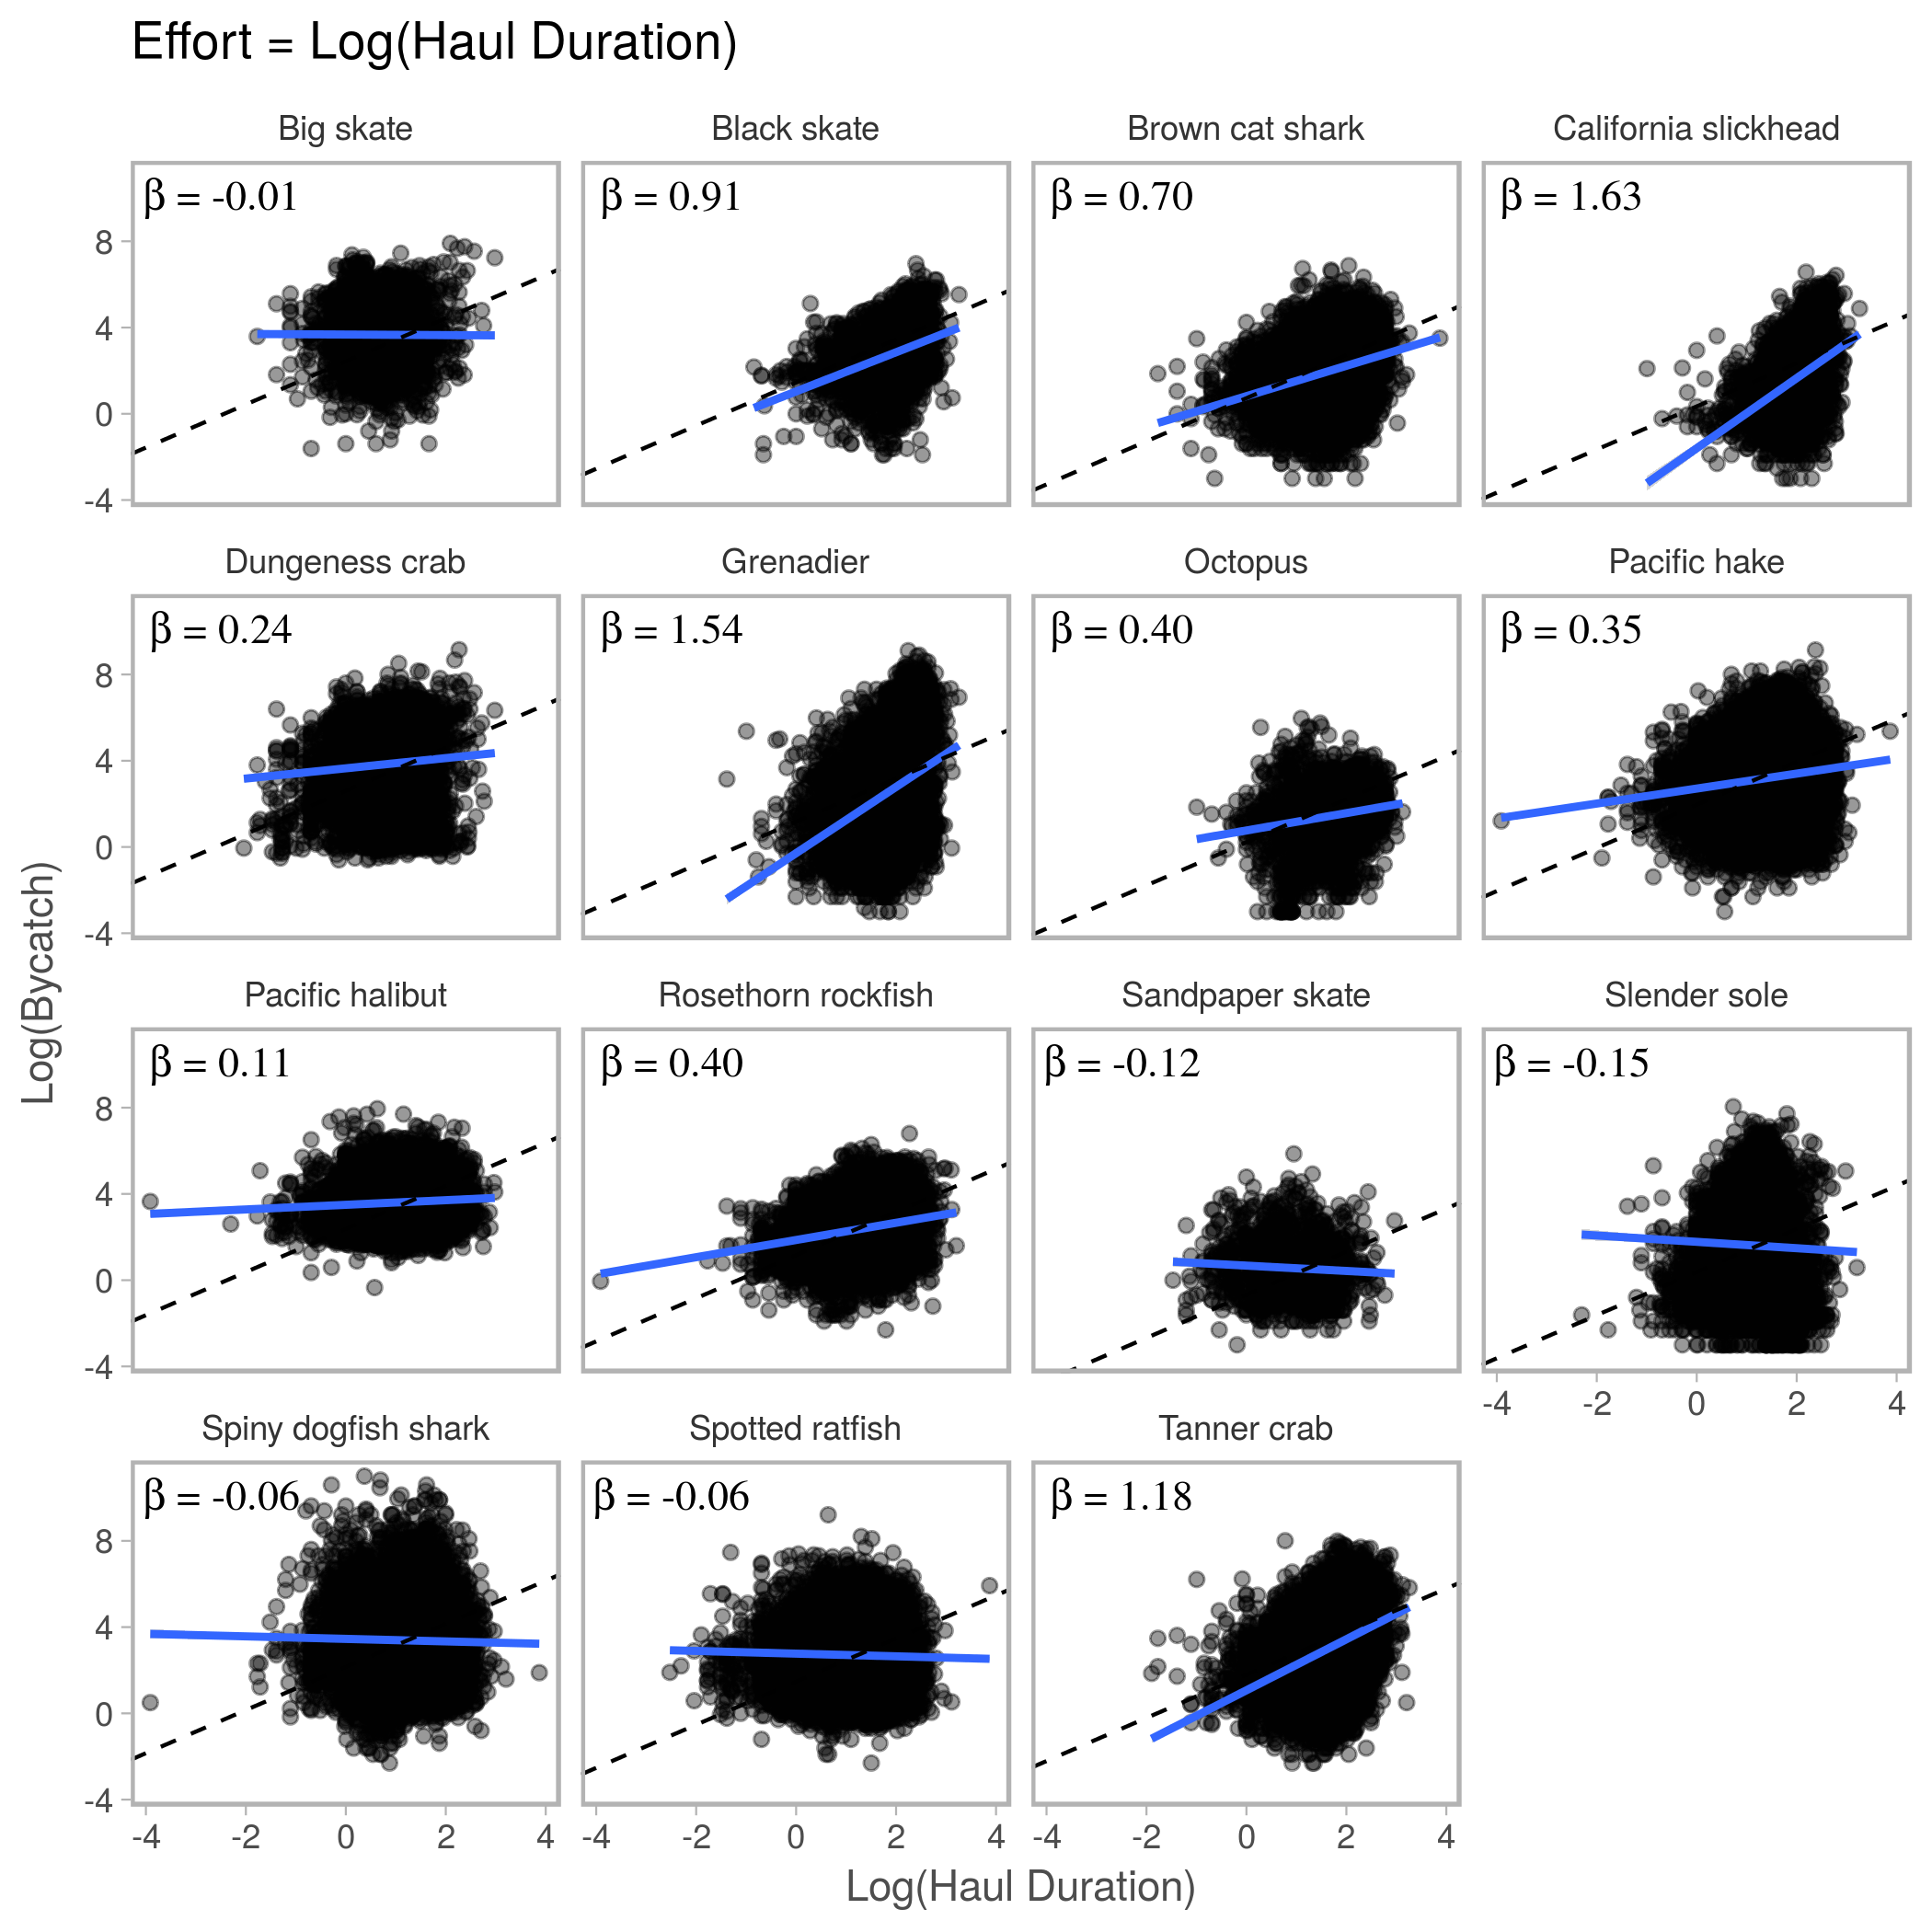
\includegraphics[width=6in]{../../figures/fig2_effort_bycatch/fig2_effort_bycatch_hauldur} 

}

\caption[Estimated relationships between fishing effort (haul duration in hours) and bycatch (kg) for 15 species analyzed in the West Coast groundfish trawl fishery.]{Estimated relationships between fishing effort (haul duration in hours) and bycatch (kg) for 15 species analyzed in the West Coast groundfish trawl fishery. The slope terms, $\beta$, of log-log linear models are exponents of an assumed power law fit to each species, $\text{Bycatch} = \alpha \text{Effort}^{\beta}$. Most $\beta$ are much less than 1, indicating the relationship between bycatch and effort is either weak or not linear. Data ($n = 35,440$) consist of observed hauls from the West Coast Groundfish Observer Program recorded from 2011 to 2015 in the area north of Cape Falcon, Oregon (45.77° N).}\label{fig:effort-bycatch-2}
\end{figure}

\pagebreak

\subsection{Figure S2}\label{figure-s2}

\begin{figure}[H]

{\centering 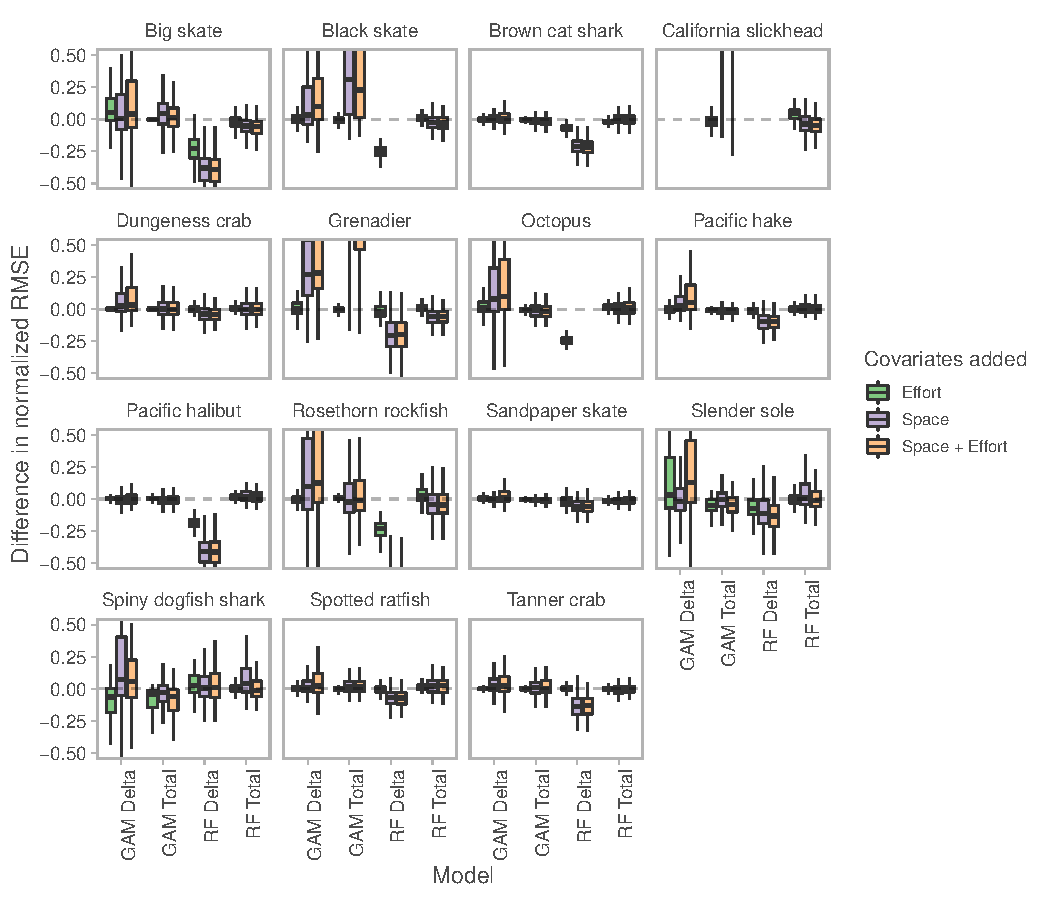
\includegraphics[width=7in]{bycatch_sim_paper_supplement_files/figure-latex/covariate-effects-1} 

}

\caption[Change in predictive performance (normalized RMSE) when adding fishing effort and spatial location as covariates in each model.]{Change in predictive performance (normalized RMSE) when adding fishing effort and spatial location as covariates in each model. For many species, adding space to the GAM-Delta and GAM-Total models led to worse predictions (positive change in RMSE, above dashed line). On the other hand, adding space to the RF-Delta model consistently improved predictions (negative change in RMSE, below dashed line). For RF-Total, including space had either slightly improved predictions or had no effect. Adding effort had little effect for nearly all species and models, and never had a larger effect than adding space.}\label{fig:covariate-effects}
\end{figure}

\pagebreak

\subsection{Figure S3}\label{figure-s3}

\begin{figure}[H]

{\centering 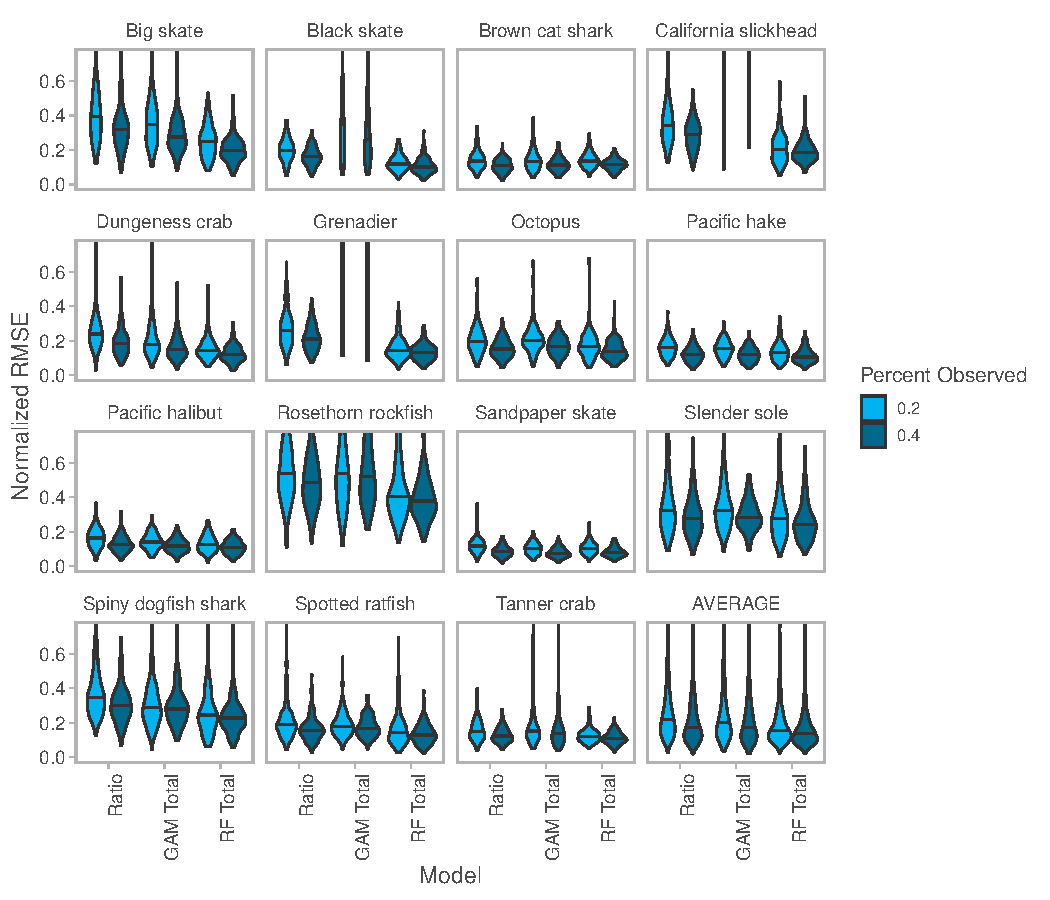
\includegraphics[width=7in]{bycatch_sim_paper_supplement_files/figure-latex/coverage-effects-1} 

}

\caption[Predictive performance (normalized RMSE) for different levels of simulated observer coverage.]{Predictive performance (normalized RMSE) for different levels of simulated observer coverage. Averaged across species, RF-Total had lower median RMSE than the ratio estimator, even at half the observer coverage (RF-Total at 20\%: 0.155, Ratio at 40\%: 0.180). GAM-Total failed to converge for 3/15 species.}\label{fig:coverage-effects}
\end{figure}

\pagebreak

\subsection{Figure S4}\label{figure-s4}

\begin{figure}[H]

{\centering 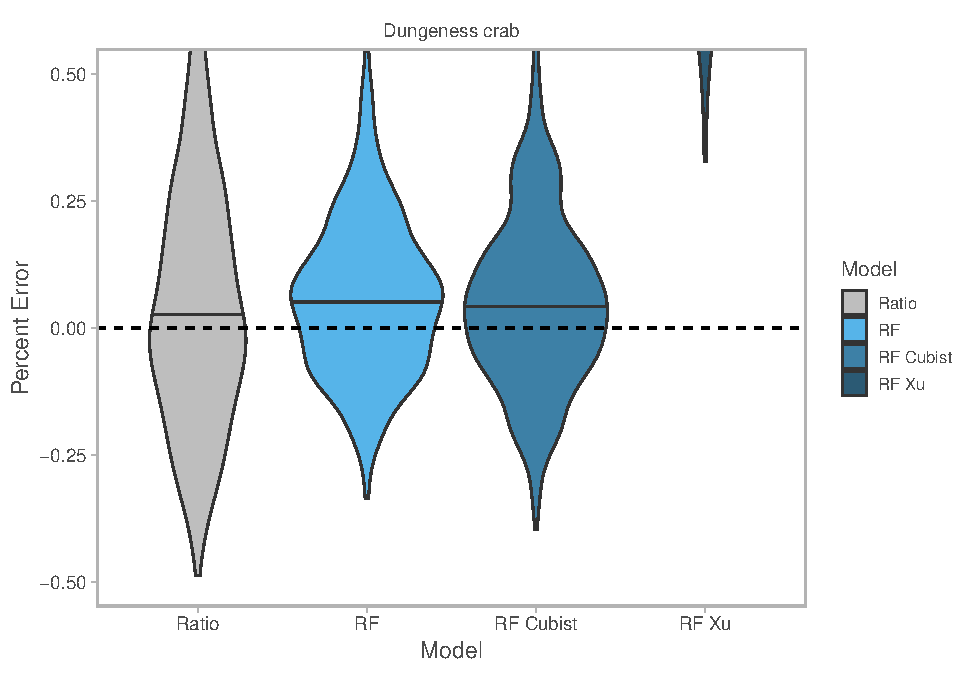
\includegraphics[width=6in]{bycatch_sim_paper_supplement_files/figure-latex/rf-cubist-1} 

}

\caption[Performance of RF bias correction methods (percent error, PE, averaged across years 2011-2015).]{Performance of RF bias correction methods applied to Dungeness Crab bycatch (percent error, PE, averaged across years 2011-2015). The ratio estimator is unbiased (median PE = 0.002). RF is positively biased (median PE = 0.055) and Cubist is less positively biased (median PE = 0.043). Cubist reduces bias by fitting a linear model in regression tree terminal nodes instead of using the data mean (Quinlan 1992, Quinlan 1993). The second method, Xu (2013), fits a second RF model to the residuals of the original RF, but this method performed poorly (median PE = 1.107, off chart).}\label{fig:rf-cubist}
\end{figure}


\end{document}
